\documentclass[twoside]{book}

% Packages required by doxygen
\usepackage{fixltx2e}
\usepackage{calc}
\usepackage{doxygen}
\usepackage[export]{adjustbox} % also loads graphicx
\usepackage{graphicx}
\usepackage[utf8]{inputenc}
\usepackage{makeidx}
\usepackage{multicol}
\usepackage{multirow}
\PassOptionsToPackage{warn}{textcomp}
\usepackage{textcomp}
\usepackage[nointegrals]{wasysym}
\usepackage[table]{xcolor}

% Font selection
\usepackage[T1]{fontenc}
\usepackage[scaled=.90]{helvet}
\usepackage{courier}
\usepackage{amssymb}
\usepackage{sectsty}
\renewcommand{\familydefault}{\sfdefault}
\allsectionsfont{%
  \fontseries{bc}\selectfont%
  \color{darkgray}%
}
\renewcommand{\DoxyLabelFont}{%
  \fontseries{bc}\selectfont%
  \color{darkgray}%
}
\newcommand{\+}{\discretionary{\mbox{\scriptsize$\hookleftarrow$}}{}{}}

% Page & text layout
\usepackage{geometry}
\geometry{%
  a4paper,%
  top=2.5cm,%
  bottom=2.5cm,%
  left=2.5cm,%
  right=2.5cm%
}
\tolerance=750
\hfuzz=15pt
\hbadness=750
\setlength{\emergencystretch}{15pt}
\setlength{\parindent}{0cm}
\setlength{\parskip}{3ex plus 2ex minus 2ex}
\makeatletter
\renewcommand{\paragraph}{%
  \@startsection{paragraph}{4}{0ex}{-1.0ex}{1.0ex}{%
    \normalfont\normalsize\bfseries\SS@parafont%
  }%
}
\renewcommand{\subparagraph}{%
  \@startsection{subparagraph}{5}{0ex}{-1.0ex}{1.0ex}{%
    \normalfont\normalsize\bfseries\SS@subparafont%
  }%
}
\makeatother

% Headers & footers
\usepackage{fancyhdr}
\pagestyle{fancyplain}
\fancyhead[LE]{\fancyplain{}{\bfseries\thepage}}
\fancyhead[CE]{\fancyplain{}{}}
\fancyhead[RE]{\fancyplain{}{\bfseries\leftmark}}
\fancyhead[LO]{\fancyplain{}{\bfseries\rightmark}}
\fancyhead[CO]{\fancyplain{}{}}
\fancyhead[RO]{\fancyplain{}{\bfseries\thepage}}
\fancyfoot[LE]{\fancyplain{}{}}
\fancyfoot[CE]{\fancyplain{}{}}
\fancyfoot[RE]{\fancyplain{}{\bfseries\scriptsize Generated by Doxygen }}
\fancyfoot[LO]{\fancyplain{}{\bfseries\scriptsize Generated by Doxygen }}
\fancyfoot[CO]{\fancyplain{}{}}
\fancyfoot[RO]{\fancyplain{}{}}
\renewcommand{\footrulewidth}{0.4pt}
\renewcommand{\chaptermark}[1]{%
  \markboth{#1}{}%
}
\renewcommand{\sectionmark}[1]{%
  \markright{\thesection\ #1}%
}

% Indices & bibliography
\usepackage{natbib}
\usepackage[titles]{tocloft}
\setcounter{tocdepth}{3}
\setcounter{secnumdepth}{5}
\makeindex

% Hyperlinks (required, but should be loaded last)
\usepackage{ifpdf}
\ifpdf
  \usepackage[pdftex,pagebackref=true]{hyperref}
\else
  \usepackage[ps2pdf,pagebackref=true]{hyperref}
\fi
\hypersetup{%
  colorlinks=true,%
  linkcolor=blue,%
  citecolor=blue,%
  unicode%
}

% Custom commands
\newcommand{\clearemptydoublepage}{%
  \newpage{\pagestyle{empty}\cleardoublepage}%
}

\usepackage{caption}
\captionsetup{labelsep=space,justification=centering,font={bf},singlelinecheck=off,skip=4pt,position=top}

%===== C O N T E N T S =====

\begin{document}

% Titlepage & ToC
\hypersetup{pageanchor=false,
             bookmarksnumbered=true,
             pdfencoding=unicode
            }
\pagenumbering{alph}
\begin{titlepage}
\vspace*{7cm}
\begin{center}%
{\Large Entities }\\
\vspace*{1cm}
{\large Generated by Doxygen 1.8.13}\\
\end{center}
\end{titlepage}
\clearemptydoublepage
\pagenumbering{roman}
\tableofcontents
\clearemptydoublepage
\pagenumbering{arabic}
\hypersetup{pageanchor=true}

%--- Begin generated contents ---
\chapter{Hierarchical Index}
\section{Class Hierarchy}
This inheritance list is sorted roughly, but not completely, alphabetically\+:\begin{DoxyCompactList}
\item \contentsline{section}{Entity}{\pageref{class_entity}}{}
\item \contentsline{section}{Entity\+Component}{\pageref{class_entity_component}}{}
\begin{DoxyCompactList}
\item \contentsline{section}{Entity\+Component\+Empty}{\pageref{class_entity_component_empty}}{}
\item \contentsline{section}{Entity\+Component\+Pos3}{\pageref{class_entity_component_pos3}}{}
\item \contentsline{section}{Entity\+Component\+Tag}{\pageref{class_entity_component_tag}}{}
\end{DoxyCompactList}
\item \contentsline{section}{Entity\+Factory}{\pageref{class_entity_factory}}{}
\item \contentsline{section}{Save\+File\+Reader}{\pageref{class_save_file_reader}}{}
\item \contentsline{section}{Save\+File\+Writer}{\pageref{class_save_file_writer}}{}
\end{DoxyCompactList}

\chapter{Class Index}
\section{Class List}
Here are the classes, structs, unions and interfaces with brief descriptions\+:\begin{DoxyCompactList}
\item\contentsline{section}{\hyperlink{class_entity}{Entity} }{\pageref{class_entity}}{}
\item\contentsline{section}{\hyperlink{class_entity_component}{Entity\+Component} }{\pageref{class_entity_component}}{}
\item\contentsline{section}{\hyperlink{class_entity_component_empty}{Entity\+Component\+Empty} }{\pageref{class_entity_component_empty}}{}
\item\contentsline{section}{\hyperlink{class_entity_component_pos3}{Entity\+Component\+Pos3} }{\pageref{class_entity_component_pos3}}{}
\item\contentsline{section}{\hyperlink{class_entity_component_tag}{Entity\+Component\+Tag} }{\pageref{class_entity_component_tag}}{}
\item\contentsline{section}{\hyperlink{class_entity_factory}{Entity\+Factory} }{\pageref{class_entity_factory}}{}
\item\contentsline{section}{\hyperlink{class_save_file_reader}{Save\+File\+Reader} }{\pageref{class_save_file_reader}}{}
\item\contentsline{section}{\hyperlink{class_save_file_writer}{Save\+File\+Writer} }{\pageref{class_save_file_writer}}{}
\end{DoxyCompactList}

\chapter{File Index}
\section{File List}
Here is a list of all documented files with brief descriptions\+:\begin{DoxyCompactList}
\item\contentsline{section}{{\bfseries entity.\+h} }{\pageref{entity_8h}}{}
\item\contentsline{section}{{\bfseries entity\+\_\+factory.\+h} }{\pageref{entity__factory_8h}}{}
\item\contentsline{section}{\hyperlink{entity__fields_8h}{entity\+\_\+fields.\+h} }{\pageref{entity__fields_8h}}{}
\item\contentsline{section}{{\bfseries file\+\_\+save.\+h} }{\pageref{file__save_8h}}{}
\end{DoxyCompactList}

\chapter{Class Documentation}
\hypertarget{class_entity}{}\section{Entity Class Reference}
\label{class_entity}\index{Entity@{Entity}}
\subsection*{Public Member Functions}
\begin{DoxyCompactItemize}
\item 
\mbox{\Hypertarget{class_entity_a0729633dfb5e5bafbc90344ebf8084e1}\label{class_entity_a0729633dfb5e5bafbc90344ebf8084e1}} 
void {\bfseries add\+Component} (\hyperlink{class_entity_component}{Entity\+Component} $\ast$comp)
\item 
\mbox{\Hypertarget{class_entity_a2b6176cc5cbdcbcf50c3e504b2d2cf1e}\label{class_entity_a2b6176cc5cbdcbcf50c3e504b2d2cf1e}} 
virtual \hyperlink{class_entity}{Entity} $\ast$ {\bfseries load} (\hyperlink{class_save_file_reader}{Save\+File\+Reader} \&sfr)
\item 
\mbox{\Hypertarget{class_entity_a50c4e0080827d7fc42d40dc183eb7226}\label{class_entity_a50c4e0080827d7fc42d40dc183eb7226}} 
virtual void {\bfseries save} (\hyperlink{class_save_file_writer}{Save\+File\+Writer} \&sfw)
\item 
\mbox{\Hypertarget{class_entity_a2d2e82ce6acc0a4c718e29563fe6cfb9}\label{class_entity_a2d2e82ce6acc0a4c718e29563fe6cfb9}} 
std\+::string {\bfseries to\+String} ()
\end{DoxyCompactItemize}


The documentation for this class was generated from the following files\+:\begin{DoxyCompactItemize}
\item 
entity.\+h\item 
entity.\+cpp\end{DoxyCompactItemize}

\hypertarget{class_entity_component}{}\section{Entity\+Component Class Reference}
\label{class_entity_component}\index{Entity\+Component@{Entity\+Component}}
Inheritance diagram for Entity\+Component\+:\begin{figure}[H]
\begin{center}
\leavevmode
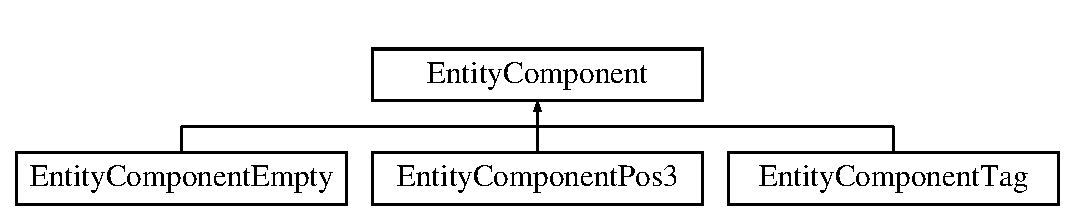
\includegraphics[height=2.000000cm]{class_entity_component}
\end{center}
\end{figure}
\subsection*{Public Member Functions}
\begin{DoxyCompactItemize}
\item 
\mbox{\Hypertarget{class_entity_component_a0c002afd63cb992b135cc8e8b6e22106}\label{class_entity_component_a0c002afd63cb992b135cc8e8b6e22106}} 
virtual \hyperlink{class_entity_component}{Entity\+Component} $\ast$ {\bfseries load} (\hyperlink{class_save_file_reader}{Save\+File\+Reader} \&sfr)
\item 
\mbox{\Hypertarget{class_entity_component_a812405a882aba0f4faa83c90995d5806}\label{class_entity_component_a812405a882aba0f4faa83c90995d5806}} 
virtual void {\bfseries save} (\hyperlink{class_save_file_writer}{Save\+File\+Writer} \&sfw)
\item 
\mbox{\Hypertarget{class_entity_component_a89789e02c5b5a6171bbafb8953f226e4}\label{class_entity_component_a89789e02c5b5a6171bbafb8953f226e4}} 
virtual std\+::string {\bfseries to\+String} ()
\end{DoxyCompactItemize}


The documentation for this class was generated from the following files\+:\begin{DoxyCompactItemize}
\item 
entity.\+h\item 
entity.\+cpp\end{DoxyCompactItemize}

\hypertarget{class_entity_component_empty}{}\section{Entity\+Component\+Empty Class Reference}
\label{class_entity_component_empty}\index{Entity\+Component\+Empty@{Entity\+Component\+Empty}}
Inheritance diagram for Entity\+Component\+Empty\+:\begin{figure}[H]
\begin{center}
\leavevmode
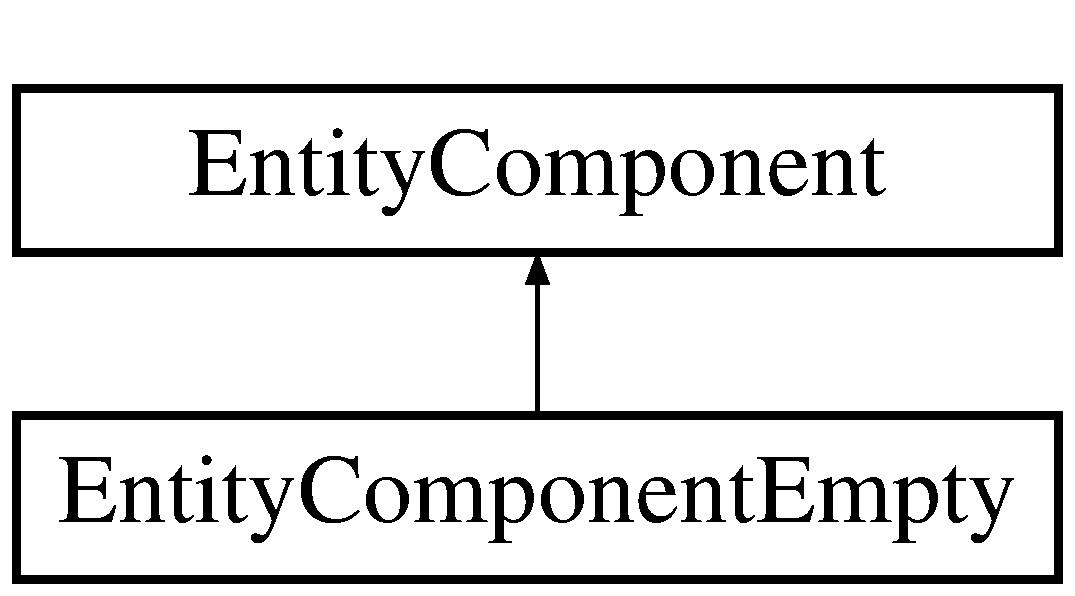
\includegraphics[height=2.000000cm]{class_entity_component_empty}
\end{center}
\end{figure}
\subsection*{Additional Inherited Members}


The documentation for this class was generated from the following file\+:\begin{DoxyCompactItemize}
\item 
main.\+cpp\end{DoxyCompactItemize}

\hypertarget{class_entity_component_pos3}{}\section{Entity\+Component\+Pos3 Class Reference}
\label{class_entity_component_pos3}\index{Entity\+Component\+Pos3@{Entity\+Component\+Pos3}}
Inheritance diagram for Entity\+Component\+Pos3\+:\begin{figure}[H]
\begin{center}
\leavevmode
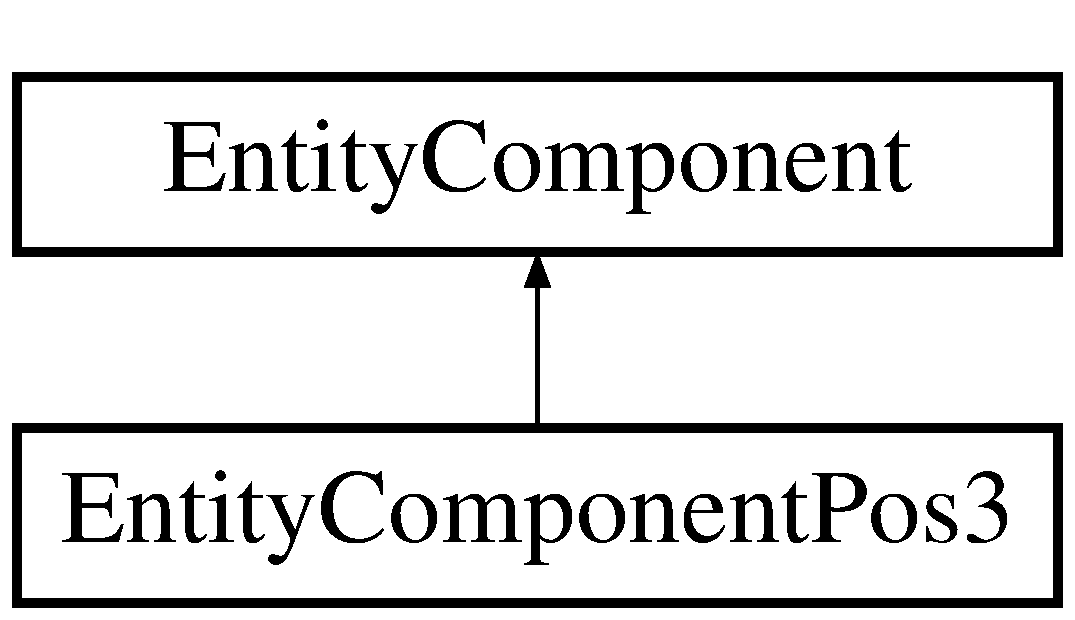
\includegraphics[height=2.000000cm]{class_entity_component_pos3}
\end{center}
\end{figure}
\subsection*{Additional Inherited Members}


The documentation for this class was generated from the following file\+:\begin{DoxyCompactItemize}
\item 
main.\+cpp\end{DoxyCompactItemize}

\hypertarget{class_entity_component_tag}{}\section{Entity\+Component\+Tag Class Reference}
\label{class_entity_component_tag}\index{Entity\+Component\+Tag@{Entity\+Component\+Tag}}
Inheritance diagram for Entity\+Component\+Tag\+:\begin{figure}[H]
\begin{center}
\leavevmode
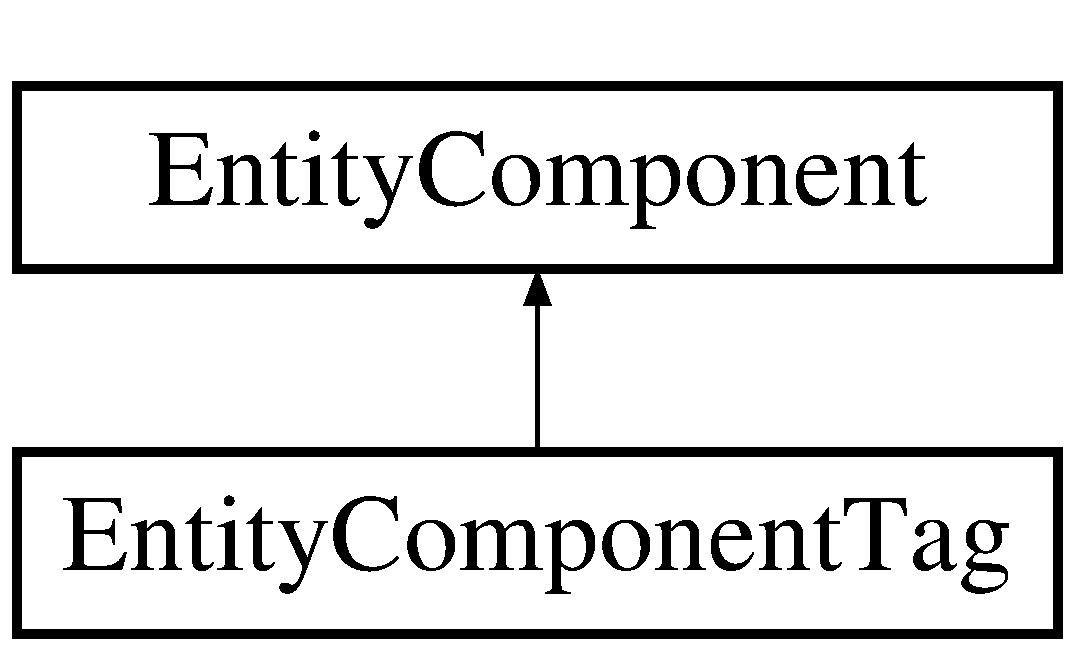
\includegraphics[height=2.000000cm]{class_entity_component_tag}
\end{center}
\end{figure}
\subsection*{Additional Inherited Members}


The documentation for this class was generated from the following file\+:\begin{DoxyCompactItemize}
\item 
main.\+cpp\end{DoxyCompactItemize}

\hypertarget{class_entity_factory}{}\section{Entity\+Factory Class Reference}
\label{class_entity_factory}\index{Entity\+Factory@{Entity\+Factory}}
\subsection*{Public Member Functions}
\begin{DoxyCompactItemize}
\item 
\mbox{\Hypertarget{class_entity_factory_a8d71e5cc38b588731169c475778ab21f}\label{class_entity_factory_a8d71e5cc38b588731169c475778ab21f}} 
void {\bfseries register\+Ent\+Comp} (std\+::string name, std\+::function$<$ \hyperlink{class_entity_component}{Entity\+Component} $\ast$()$>$ construction\+\_\+func)
\item 
\mbox{\Hypertarget{class_entity_factory_a2ab1d07653d50c80a77114566a9c19c7}\label{class_entity_factory_a2ab1d07653d50c80a77114566a9c19c7}} 
\hyperlink{class_entity_component}{Entity\+Component} $\ast$ {\bfseries construct\+Ent\+Comp} (std\+::string name)
\item 
\mbox{\Hypertarget{class_entity_factory_ac516b734bae6d5a15c8b491bc7e80ae7}\label{class_entity_factory_ac516b734bae6d5a15c8b491bc7e80ae7}} 
std\+::vector$<$ std\+::string $>$ $\ast$ {\bfseries get\+Ent\+Comps} ()
\end{DoxyCompactItemize}
\subsection*{Static Public Attributes}
\begin{DoxyCompactItemize}
\item 
\mbox{\Hypertarget{class_entity_factory_a5e193c2faa26b7cfb2ae85074d662749}\label{class_entity_factory_a5e193c2faa26b7cfb2ae85074d662749}} 
static \hyperlink{class_entity_factory}{Entity\+Factory} $\ast$ {\bfseries inst}
\end{DoxyCompactItemize}


The documentation for this class was generated from the following files\+:\begin{DoxyCompactItemize}
\item 
entity\+\_\+factory.\+h\item 
entity\+\_\+factory.\+cpp\end{DoxyCompactItemize}

\hypertarget{class_save_file_reader}{}\section{Save\+File\+Reader Class Reference}
\label{class_save_file_reader}\index{Save\+File\+Reader@{Save\+File\+Reader}}


{\ttfamily \#include $<$file\+\_\+save.\+h$>$}

\subsection*{Public Member Functions}
\begin{DoxyCompactItemize}
\item 
\mbox{\Hypertarget{class_save_file_reader_a266182124313a80df2ff69b4d5b72645}\label{class_save_file_reader_a266182124313a80df2ff69b4d5b72645}} 
{\bfseries Save\+File\+Reader} (std\+::string fname)
\item 
\mbox{\Hypertarget{class_save_file_reader_a956edd660e6cb542ed3bcdb206c9cca4}\label{class_save_file_reader_a956edd660e6cb542ed3bcdb206c9cca4}} 
void {\bfseries close} ()
\item 
std\+::string \hyperlink{class_save_file_reader_afb12610d8d9f39adc1c3db60ae8afda3}{get\+Ent\+Comp\+Name} (unsigned int ind)
\item 
void \hyperlink{class_save_file_reader_a6fe25b46135c278be875bec0ef19bdf3}{read\+Ent\+Comp\+Map} ()
\item 
{\footnotesize template$<$class T $>$ }\\T \hyperlink{class_save_file_reader_aaacf90b2df172da6dbd4f372c57df0a2}{read} ()
\item 
std\+::vector$<$ char $>$ $\ast$ \hyperlink{class_save_file_reader_a7272a5a3877eb91ed668b879e7f66398}{read\+\_\+array} (size\+\_\+t bytes)
\end{DoxyCompactItemize}


\subsection{Detailed Description}
Reads binary files generated by \hyperlink{class_save_file_writer}{Save\+File\+Writer}. For file format details, see the class definition of \hyperlink{class_save_file_writer}{Save\+File\+Writer}. 

\subsection{Member Function Documentation}
\mbox{\Hypertarget{class_save_file_reader_afb12610d8d9f39adc1c3db60ae8afda3}\label{class_save_file_reader_afb12610d8d9f39adc1c3db60ae8afda3}} 
\index{Save\+File\+Reader@{Save\+File\+Reader}!get\+Ent\+Comp\+Name@{get\+Ent\+Comp\+Name}}
\index{get\+Ent\+Comp\+Name@{get\+Ent\+Comp\+Name}!Save\+File\+Reader@{Save\+File\+Reader}}
\subsubsection{\texorpdfstring{get\+Ent\+Comp\+Name()}{getEntCompName()}}
{\footnotesize\ttfamily std\+::string Save\+File\+Reader\+::get\+Ent\+Comp\+Name (\begin{DoxyParamCaption}\item[{unsigned int}]{ind }\end{DoxyParamCaption})\hspace{0.3cm}{\ttfamily [inline]}}

Gets the class name with the supplied alias in the file. \mbox{\Hypertarget{class_save_file_reader_aaacf90b2df172da6dbd4f372c57df0a2}\label{class_save_file_reader_aaacf90b2df172da6dbd4f372c57df0a2}} 
\index{Save\+File\+Reader@{Save\+File\+Reader}!read@{read}}
\index{read@{read}!Save\+File\+Reader@{Save\+File\+Reader}}
\subsubsection{\texorpdfstring{read()}{read()}}
{\footnotesize\ttfamily template$<$class T $>$ \\
T Save\+File\+Reader\+::read (\begin{DoxyParamCaption}{ }\end{DoxyParamCaption})\hspace{0.3cm}{\ttfamily [inline]}}

Reads a variable of type T from the file. \mbox{\Hypertarget{class_save_file_reader_a7272a5a3877eb91ed668b879e7f66398}\label{class_save_file_reader_a7272a5a3877eb91ed668b879e7f66398}} 
\index{Save\+File\+Reader@{Save\+File\+Reader}!read\+\_\+array@{read\+\_\+array}}
\index{read\+\_\+array@{read\+\_\+array}!Save\+File\+Reader@{Save\+File\+Reader}}
\subsubsection{\texorpdfstring{read\+\_\+array()}{read\_array()}}
{\footnotesize\ttfamily std\+::vector$<$char$>$$\ast$ Save\+File\+Reader\+::read\+\_\+array (\begin{DoxyParamCaption}\item[{size\+\_\+t}]{bytes }\end{DoxyParamCaption})\hspace{0.3cm}{\ttfamily [inline]}}

Reads an array with a size of \textquotesingle{}bytes\textquotesingle{} bytes. The size of the array is generally written before the array as a size\+\_\+t. \mbox{\Hypertarget{class_save_file_reader_a6fe25b46135c278be875bec0ef19bdf3}\label{class_save_file_reader_a6fe25b46135c278be875bec0ef19bdf3}} 
\index{Save\+File\+Reader@{Save\+File\+Reader}!read\+Ent\+Comp\+Map@{read\+Ent\+Comp\+Map}}
\index{read\+Ent\+Comp\+Map@{read\+Ent\+Comp\+Map}!Save\+File\+Reader@{Save\+File\+Reader}}
\subsubsection{\texorpdfstring{read\+Ent\+Comp\+Map()}{readEntCompMap()}}
{\footnotesize\ttfamily void Save\+File\+Reader\+::read\+Ent\+Comp\+Map (\begin{DoxyParamCaption}{ }\end{DoxyParamCaption})}

Reads the \hyperlink{class_entity_component}{Entity\+Component} map from the top of the file. 

The documentation for this class was generated from the following files\+:\begin{DoxyCompactItemize}
\item 
file\+\_\+save.\+h\item 
file\+\_\+save.\+cpp\end{DoxyCompactItemize}

\hypertarget{class_save_file_writer}{}\section{Save\+File\+Writer Class Reference}
\label{class_save_file_writer}\index{Save\+File\+Writer@{Save\+File\+Writer}}


{\ttfamily \#include $<$file\+\_\+save.\+h$>$}

\subsection*{Public Member Functions}
\begin{DoxyCompactItemize}
\item 
\mbox{\Hypertarget{class_save_file_writer_afc1540e5b1b66a18f8d3ed78d7013748}\label{class_save_file_writer_afc1540e5b1b66a18f8d3ed78d7013748}} 
{\bfseries Save\+File\+Writer} (std\+::string fname)
\item 
\mbox{\Hypertarget{class_save_file_writer_a0c174fe28dc4070a9c71c78ede21a91c}\label{class_save_file_writer_a0c174fe28dc4070a9c71c78ede21a91c}} 
void {\bfseries close} ()
\item 
unsigned int \hyperlink{class_save_file_writer_aa5f3b020a4d93f42f274d4c5d7f10b8c}{get\+Ent\+Comp\+Index} (std\+::string entcomp)
\item 
void \hyperlink{class_save_file_writer_a3b6359fa30469f5ae518eaf009951e05}{write\+Ent\+Comp\+Map} (std\+::vector$<$ std\+::string $>$ $\ast$entcomps)
\item 
{\footnotesize template$<$class T $>$ }\\void \hyperlink{class_save_file_writer_a665e53cc0c04489c5b0872b3f8cd7218}{write} (T t)
\item 
{\footnotesize template$<$class T $>$ }\\void \hyperlink{class_save_file_writer_a314ad7bcf58b24885ec3501d2fa206e5}{write\+\_\+array} (T $\ast$t, size\+\_\+t bytes)
\end{DoxyCompactItemize}


\subsection{Detailed Description}
Writes \hyperlink{class_entity}{Entity} data to a binary save file. Format\+:
\begin{DoxyItemize}
\item \hyperlink{class_entity_component}{Entity\+Component} map (\+::entcompmap) to map class names onto unsigned integers, giving \hyperlink{class_entity_component}{Entity\+Component} subclasses \textquotesingle{}aliases\textquotesingle{} so that they can be referenced with a simple unsigned int.
\item A 0x01 character to signal the end of the block.
\item Each \hyperlink{class_entity}{Entity} is written to the file as follows\+:
\begin{DoxyItemize}
\item An unsigned int detailing how many Entity\+Components it contains.
\item Each component in turn.
\end{DoxyItemize}
\item (Unimplemented as currently only one entity can be saved and loaded back properly) A 0x01 character to signal the end of the block. 
\end{DoxyItemize}

\subsection{Member Function Documentation}
\mbox{\Hypertarget{class_save_file_writer_aa5f3b020a4d93f42f274d4c5d7f10b8c}\label{class_save_file_writer_aa5f3b020a4d93f42f274d4c5d7f10b8c}} 
\index{Save\+File\+Writer@{Save\+File\+Writer}!get\+Ent\+Comp\+Index@{get\+Ent\+Comp\+Index}}
\index{get\+Ent\+Comp\+Index@{get\+Ent\+Comp\+Index}!Save\+File\+Writer@{Save\+File\+Writer}}
\subsubsection{\texorpdfstring{get\+Ent\+Comp\+Index()}{getEntCompIndex()}}
{\footnotesize\ttfamily unsigned int Save\+File\+Writer\+::get\+Ent\+Comp\+Index (\begin{DoxyParamCaption}\item[{std\+::string}]{entcomp }\end{DoxyParamCaption})}

Gets the alias of an \hyperlink{class_entity_component}{Entity\+Component} subclass\textquotesingle{} name. This alias is used in the save file to prefix the \hyperlink{class_entity_component}{Entity\+Component} so that we know what class it is when loading the file. \mbox{\Hypertarget{class_save_file_writer_a665e53cc0c04489c5b0872b3f8cd7218}\label{class_save_file_writer_a665e53cc0c04489c5b0872b3f8cd7218}} 
\index{Save\+File\+Writer@{Save\+File\+Writer}!write@{write}}
\index{write@{write}!Save\+File\+Writer@{Save\+File\+Writer}}
\subsubsection{\texorpdfstring{write()}{write()}}
{\footnotesize\ttfamily template$<$class T $>$ \\
void Save\+File\+Writer\+::write (\begin{DoxyParamCaption}\item[{T}]{t }\end{DoxyParamCaption})\hspace{0.3cm}{\ttfamily [inline]}}

Writes a variable to the file. \mbox{\Hypertarget{class_save_file_writer_a314ad7bcf58b24885ec3501d2fa206e5}\label{class_save_file_writer_a314ad7bcf58b24885ec3501d2fa206e5}} 
\index{Save\+File\+Writer@{Save\+File\+Writer}!write\+\_\+array@{write\+\_\+array}}
\index{write\+\_\+array@{write\+\_\+array}!Save\+File\+Writer@{Save\+File\+Writer}}
\subsubsection{\texorpdfstring{write\+\_\+array()}{write\_array()}}
{\footnotesize\ttfamily template$<$class T $>$ \\
void Save\+File\+Writer\+::write\+\_\+array (\begin{DoxyParamCaption}\item[{T $\ast$}]{t,  }\item[{size\+\_\+t}]{bytes }\end{DoxyParamCaption})\hspace{0.3cm}{\ttfamily [inline]}}

Writes an array to the file. Generally the size of the array should be written to the file first, as a size\+\_\+t type. \mbox{\Hypertarget{class_save_file_writer_a3b6359fa30469f5ae518eaf009951e05}\label{class_save_file_writer_a3b6359fa30469f5ae518eaf009951e05}} 
\index{Save\+File\+Writer@{Save\+File\+Writer}!write\+Ent\+Comp\+Map@{write\+Ent\+Comp\+Map}}
\index{write\+Ent\+Comp\+Map@{write\+Ent\+Comp\+Map}!Save\+File\+Writer@{Save\+File\+Writer}}
\subsubsection{\texorpdfstring{write\+Ent\+Comp\+Map()}{writeEntCompMap()}}
{\footnotesize\ttfamily void Save\+File\+Writer\+::write\+Ent\+Comp\+Map (\begin{DoxyParamCaption}\item[{std\+::vector$<$ std\+::string $>$ $\ast$}]{entcomps }\end{DoxyParamCaption})}

Writes the map of \hyperlink{class_entity_component}{Entity\+Component} subclasses into the file. This is followed by a 0x01 character to signal the end of the block. 

The documentation for this class was generated from the following files\+:\begin{DoxyCompactItemize}
\item 
file\+\_\+save.\+h\item 
file\+\_\+save.\+cpp\end{DoxyCompactItemize}

\chapter{File Documentation}
\hypertarget{entity__fields_8h}{}\section{entity\+\_\+fields.\+h File Reference}
\label{entity__fields_8h}\index{entity\+\_\+fields.\+h@{entity\+\_\+fields.\+h}}
{\ttfamily \#include $<$string$>$}\newline
{\ttfamily \#include $<$sstream$>$}\newline
\subsection*{Macros}
\begin{DoxyCompactItemize}
\item 
\#define {\bfseries E\+N\+T\+\_\+\+R\+E\+G\+I\+S\+T\+E\+R\+\_\+\+F\+I\+E\+L\+D\+S\+\_\+0}(name)
\item 
\#define {\bfseries E\+N\+T\+\_\+\+R\+E\+G\+I\+S\+T\+E\+R\+\_\+\+F\+I\+E\+L\+D\+S\+\_\+1}(name,  type0,  var0)
\item 
\mbox{\Hypertarget{entity__fields_8h_a10c6634ceaace6f5cd200f8461f2c5a9}\label{entity__fields_8h_a10c6634ceaace6f5cd200f8461f2c5a9}} 
\#define {\bfseries E\+N\+T\+\_\+\+R\+E\+G\+I\+S\+T\+E\+R\+\_\+\+F\+I\+E\+L\+D\+S\+\_\+2}(name,  type0,  var0,  type1,  var1)
\item 
\mbox{\Hypertarget{entity__fields_8h_a1c82330cfb4d85995d85f0989b748acb}\label{entity__fields_8h_a1c82330cfb4d85995d85f0989b748acb}} 
\#define {\bfseries E\+N\+T\+\_\+\+R\+E\+G\+I\+S\+T\+E\+R\+\_\+\+F\+I\+E\+L\+D\+S\+\_\+3}(name,  type0,  var0,  type1,  var1,  type2,  var2)
\item 
\mbox{\Hypertarget{entity__fields_8h_a6f8fa5e3e6c05b608d6afe5c8a0925e2}\label{entity__fields_8h_a6f8fa5e3e6c05b608d6afe5c8a0925e2}} 
\#define {\bfseries E\+N\+T\+\_\+\+R\+E\+G\+I\+S\+T\+E\+R\+\_\+\+F\+I\+E\+L\+D\+S\+\_\+4}(name,  type0,  var0,  type1,  var1,  type2,  var2,  type3,  var3)
\item 
\mbox{\Hypertarget{entity__fields_8h_a935d63c11abf15b1924e2a3142b27044}\label{entity__fields_8h_a935d63c11abf15b1924e2a3142b27044}} 
\#define {\bfseries E\+N\+T\+\_\+\+R\+E\+G\+I\+S\+T\+E\+R\+\_\+\+F\+I\+E\+L\+D\+S\+\_\+5}(name,  type0,  var0,  type1,  var1,  type2,  var2,  type3,  var3,  type4,  var4)
\item 
\mbox{\Hypertarget{entity__fields_8h_a0212a5545459a6caca8b34ce4eedeb29}\label{entity__fields_8h_a0212a5545459a6caca8b34ce4eedeb29}} 
\#define {\bfseries E\+N\+T\+\_\+\+R\+E\+G\+I\+S\+T\+E\+R\+\_\+\+F\+I\+E\+L\+D\+S\+\_\+6}(name,  type0,  var0,  type1,  var1,  type2,  var2,  type3,  var3,  type4,  var4,  type5,  var5)
\item 
\mbox{\Hypertarget{entity__fields_8h_af5f5d0d51bdea3f5b7c7be810cde48a2}\label{entity__fields_8h_af5f5d0d51bdea3f5b7c7be810cde48a2}} 
\#define {\bfseries E\+N\+T\+\_\+\+R\+E\+G\+I\+S\+T\+E\+R\+\_\+\+F\+I\+E\+L\+D\+S\+\_\+7}(name,  type0,  var0,  type1,  var1,  type2,  var2,  type3,  var3,  type4,  var4,  type5,  var5,  type6,  var6)
\item 
\mbox{\Hypertarget{entity__fields_8h_a66c1d3892353efbb61e13641d731b332}\label{entity__fields_8h_a66c1d3892353efbb61e13641d731b332}} 
\#define {\bfseries E\+N\+T\+\_\+\+R\+E\+G\+I\+S\+T\+E\+R\+\_\+\+F\+I\+E\+L\+D\+S\+\_\+8}(name,  type0,  var0,  type1,  var1,  type2,  var2,  type3,  var3,  type4,  var4,  type5,  var5,  type6,  var6,  type7,  var7)
\item 
\mbox{\Hypertarget{entity__fields_8h_a78aec6adb0f7edc4139ff0fddd38c3a7}\label{entity__fields_8h_a78aec6adb0f7edc4139ff0fddd38c3a7}} 
\#define {\bfseries E\+N\+T\+\_\+\+R\+E\+G\+I\+S\+T\+E\+R\+\_\+\+F\+I\+E\+L\+D\+S\+\_\+9}(name,  type0,  var0,  type1,  var1,  type2,  var2,  type3,  var3,  type4,  var4,  type5,  var5,  type6,  var6,  type7,  var7,  type8,  var8)
\item 
\mbox{\Hypertarget{entity__fields_8h_ad21f866f61821352541e40897fbf93d2}\label{entity__fields_8h_ad21f866f61821352541e40897fbf93d2}} 
\#define {\bfseries E\+N\+T\+\_\+\+R\+E\+G\+I\+S\+T\+E\+R\+\_\+\+F\+I\+E\+L\+D\+S\+\_\+10}(name,  type0,  var0,  type1,  var1,  type2,  var2,  type3,  var3,  type4,  var4,  type5,  var5,  type6,  var6,  type7,  var7,  type8,  var8,  type9,  var9)
\end{DoxyCompactItemize}
\subsection*{Functions}
\begin{DoxyCompactItemize}
\item 
\mbox{\Hypertarget{entity__fields_8h_a31519e1bf8d0c893728dfebd261d8aab}\label{entity__fields_8h_a31519e1bf8d0c893728dfebd261d8aab}} 
size\+\_\+t {\bfseries \+\_\+\+\_\+ent\+\_\+str\+\_\+len} (void $\ast$ptr)
\item 
\mbox{\Hypertarget{entity__fields_8h_aacf5438fbc76ffc10527dd20b2c1aafd}\label{entity__fields_8h_aacf5438fbc76ffc10527dd20b2c1aafd}} 
void {\bfseries \+\_\+\+\_\+ent\+\_\+str\+\_\+set} (void $\ast$ptr, std\+::string \&str)
\item 
\mbox{\Hypertarget{entity__fields_8h_a10fd0e0654f1008f3e5fc32ff90d6522}\label{entity__fields_8h_a10fd0e0654f1008f3e5fc32ff90d6522}} 
const char $\ast$ {\bfseries \+\_\+\+\_\+ent\+\_\+str\+\_\+cstr} (void $\ast$ptr)
\item 
\mbox{\Hypertarget{entity__fields_8h_a2e4dbbd144939ea4da8a3a05944269fc}\label{entity__fields_8h_a2e4dbbd144939ea4da8a3a05944269fc}} 
std\+::string {\bfseries \+\_\+\+\_\+ent\+\_\+str\+\_\+tostr} (void $\ast$ptr)
\item 
\mbox{\Hypertarget{entity__fields_8h_a59cf4d7f3433c66030aaef0d5cd05b08}\label{entity__fields_8h_a59cf4d7f3433c66030aaef0d5cd05b08}} 
{\footnotesize template$<$typename T $>$ }\\std\+::string {\bfseries \+\_\+\+\_\+ent\+\_\+tostr\+\_\+not\+\_\+str} (T val)
\end{DoxyCompactItemize}


\subsection{Detailed Description}
Generated by entity\+\_\+fields\+\_\+generator.\+py. This file contains macros named \+::\+E\+N\+T\+\_\+\+R\+E\+G\+I\+S\+T\+E\+R\+\_\+\+F\+I\+E\+L\+D\+S\+\_\+0 through 10. These are intended to be used in the class definition of any user-\/defined \hyperlink{class_entity_component}{Entity\+Component}. The macros declare the variables passed to it (with access modifier \textquotesingle{}public\textquotesingle{}) and override the functions Entity\+Component\+::save() and Entity\+Component\+::load() by automatically setting the fields or writing them to the binary save file. Any fields which do not require saving (e.\+g. pointers) should be omitted from declaration in these macros. 

\subsection{Macro Definition Documentation}
\mbox{\Hypertarget{entity__fields_8h_a18a7d01e6d056619ba22b811fbe15e12}\label{entity__fields_8h_a18a7d01e6d056619ba22b811fbe15e12}} 
\index{entity\+\_\+fields.\+h@{entity\+\_\+fields.\+h}!E\+N\+T\+\_\+\+R\+E\+G\+I\+S\+T\+E\+R\+\_\+\+F\+I\+E\+L\+D\+S\+\_\+0@{E\+N\+T\+\_\+\+R\+E\+G\+I\+S\+T\+E\+R\+\_\+\+F\+I\+E\+L\+D\+S\+\_\+0}}
\index{E\+N\+T\+\_\+\+R\+E\+G\+I\+S\+T\+E\+R\+\_\+\+F\+I\+E\+L\+D\+S\+\_\+0@{E\+N\+T\+\_\+\+R\+E\+G\+I\+S\+T\+E\+R\+\_\+\+F\+I\+E\+L\+D\+S\+\_\+0}!entity\+\_\+fields.\+h@{entity\+\_\+fields.\+h}}
\subsubsection{\texorpdfstring{E\+N\+T\+\_\+\+R\+E\+G\+I\+S\+T\+E\+R\+\_\+\+F\+I\+E\+L\+D\+S\+\_\+0}{ENT\_REGISTER\_FIELDS\_0}}
{\footnotesize\ttfamily \#define E\+N\+T\+\_\+\+R\+E\+G\+I\+S\+T\+E\+R\+\_\+\+F\+I\+E\+L\+D\+S\+\_\+0(\begin{DoxyParamCaption}\item[{}]{name }\end{DoxyParamCaption})}

{\bfseries Value\+:}
\begin{DoxyCode}
\textcolor{keyword}{public}: \(\backslash\)
    virtual \textcolor{keyword}{inline} std::string toString()\textcolor{keyword}{ override }\{ \(\backslash\)
        return #name ## \textcolor{stringliteral}{" ( )"}; \(\backslash\)
    \} \(\backslash\)
    virtual \textcolor{keyword}{inline} \textcolor{keywordtype}{void} save(\hyperlink{class_save_file_writer}{SaveFileWriter}& sfw)\textcolor{keyword}{ override }\{ \(\backslash\)
        sfw.write<\textcolor{keywordtype}{unsigned} \textcolor{keywordtype}{int}>(sfw.\hyperlink{class_save_file_writer_aa5f3b020a4d93f42f274d4c5d7f10b8c}{getEntCompIndex}(#name)); \(\backslash\)
    \}
\end{DoxyCode}
\mbox{\Hypertarget{entity__fields_8h_a0324022bee0b1c4025ccec202fe88b0c}\label{entity__fields_8h_a0324022bee0b1c4025ccec202fe88b0c}} 
\index{entity\+\_\+fields.\+h@{entity\+\_\+fields.\+h}!E\+N\+T\+\_\+\+R\+E\+G\+I\+S\+T\+E\+R\+\_\+\+F\+I\+E\+L\+D\+S\+\_\+1@{E\+N\+T\+\_\+\+R\+E\+G\+I\+S\+T\+E\+R\+\_\+\+F\+I\+E\+L\+D\+S\+\_\+1}}
\index{E\+N\+T\+\_\+\+R\+E\+G\+I\+S\+T\+E\+R\+\_\+\+F\+I\+E\+L\+D\+S\+\_\+1@{E\+N\+T\+\_\+\+R\+E\+G\+I\+S\+T\+E\+R\+\_\+\+F\+I\+E\+L\+D\+S\+\_\+1}!entity\+\_\+fields.\+h@{entity\+\_\+fields.\+h}}
\subsubsection{\texorpdfstring{E\+N\+T\+\_\+\+R\+E\+G\+I\+S\+T\+E\+R\+\_\+\+F\+I\+E\+L\+D\+S\+\_\+1}{ENT\_REGISTER\_FIELDS\_1}}
{\footnotesize\ttfamily \#define E\+N\+T\+\_\+\+R\+E\+G\+I\+S\+T\+E\+R\+\_\+\+F\+I\+E\+L\+D\+S\+\_\+1(\begin{DoxyParamCaption}\item[{}]{name,  }\item[{}]{type0,  }\item[{}]{var0 }\end{DoxyParamCaption})}

{\bfseries Value\+:}
\begin{DoxyCode}
\textcolor{keyword}{public}: \(\backslash\)
    type0 var0; \(\backslash\)
    virtual \textcolor{keyword}{inline} std::string toString()\textcolor{keyword}{ override }\{ \(\backslash\)
        return #name ## \textcolor{stringliteral}{" ( "} + \_\_ent\_tostr\_not\_str<type0>(var0) + \textcolor{stringliteral}{" "} \textcolor{stringliteral}{")"};\(\backslash\)
    \}\(\backslash\)
    virtual \textcolor{keyword}{inline} \textcolor{keywordtype}{void} save(\hyperlink{class_save_file_writer}{SaveFileWriter}& sfw)\textcolor{keyword}{ override }\{ \(\backslash\)
        sfw.write<\textcolor{keywordtype}{unsigned} \textcolor{keywordtype}{int}>(sfw.\hyperlink{class_save_file_writer_aa5f3b020a4d93f42f274d4c5d7f10b8c}{getEntCompIndex}(#name));\(\backslash\)
        if (#type0 == \textcolor{stringliteral}{"std::string"} || #type0 == \textcolor{stringliteral}{"string"}) \{ \(\backslash\)
            sfw.write<\textcolor{keywordtype}{size\_t}>(\_\_ent\_str\_len(&var0)); \(\backslash\)
            sfw.write\_array<\textcolor{keywordtype}{char}>(\textcolor{keyword}{const\_cast<}\textcolor{keywordtype}{char}*\textcolor{keyword}{>}(\_\_ent\_str\_cstr(&var0)), \_\_ent\_str\_len(&var0)); \(\backslash\)
        \} \(\backslash\)
        else \(\backslash\)
            sfw.write<type0>(var0); \(\backslash\)
    \} \(\backslash\)
    virtual \textcolor{keyword}{inline} \hyperlink{class_entity_component}{EntityComponent}* load(\hyperlink{class_save_file_reader}{SaveFileReader}& sfr)\textcolor{keyword}{ override }\{ \(\backslash\)
        if (#type0 == \textcolor{stringliteral}{"std::string"} || #type0 == \textcolor{stringliteral}{"string"}) \{ \(\backslash\)
            size\_t size = sfr.\hyperlink{class_save_file_reader_aaacf90b2df172da6dbd4f372c57df0a2}{read}<\textcolor{keywordtype}{size\_t}>(); \(\backslash\)
            auto vec = sfr.\hyperlink{class_save_file_reader_a7272a5a3877eb91ed668b879e7f66398}{read\_array}(size); \(\backslash\)
            \_\_ent\_str\_set(&var0, std::string(&(*vec)[0], &(*vec)[0] + size)); \(\backslash\)
            delete vec; \(\backslash\)
        \} \(\backslash\)
        else \(\backslash\)
            var0 = sfr.\hyperlink{class_save_file_reader_aaacf90b2df172da6dbd4f372c57df0a2}{read}<type0>(); \(\backslash\)
        return \textcolor{keyword}{this}; \(\backslash\)
    \}
\end{DoxyCode}

%--- End generated contents ---

% Index
\backmatter
\newpage
\phantomsection
\clearemptydoublepage
\addcontentsline{toc}{chapter}{Index}
\printindex

\end{document}
